\chapter{膨脹宇宙的幾何}

重點在於膨脹宇宙及其幾何。我們要先說明空間膨脹的意義，再探討是什麼驅動了膨脹。牛頓力學\(F=ma\)宇宙學會在稍後討論；接著才會把幾何與動力學結合，建立完整的 Friedmann--Robertson--Walker 架構。

\section{膨脹直線上的共動座標}

先從最簡單的例子開始：一維空間，而不是時空。想像一條無限長的直線，上面有等間距排列的星系。座標 \(x\) 此時還不表示物理距離，只用來標記星系。可以把 \(x\) 想成某個星系的名稱；即使整個排列伸展或收縮，這個名稱仍附著在該星系上。

設從標記為 \(x=0\) 的星系到標記為 \(x=1\) 的星系，其物理距離為 \(a\)。那麼，任意兩個星系之間的物理距離為
\begin{equation}
d=a\,\Delta x.
\end{equation}
座標差 \(\Delta x\) 只是標籤之間的差值。因子 \(a\) 會把這個標籤差值轉換成以米尺量得的實際距離。

現在把這條直線想像成一根正在伸展的彈性線。標籤仍隨星系移動，但相鄰星系之間的距離會隨時間改變。同樣的關係式變成
\begin{equation}
d(t)=a(t)\,\Delta x.
\end{equation}
在這個階段，均勻性只表示相鄰星系在各處的間距都相等，儘管這個共同間距可能隨時間改變。

\section{哈勃定律與中心的不存在}

若要找出兩個固定星系的相對速度，就固定這一對星系，使 \(\Delta x\) 不隨時間改變。微分後得到
\begin{align}
\dot d &= \dot a\,\Delta x \\
       &= \frac{\dot a}{a}\,a\,\Delta x \\
       &= \frac{\dot a}{a}\,d.
\end{align}
定義
\begin{equation}
H(t)\equiv \frac{\dot a}{a},
\end{equation}
則有
\begin{equation}
\dot d = H(t)\,d.
\end{equation}
這就是哈勃定律。

歷史上使用的「``哈勃常數''」一詞容易造成誤解。這個量在空間中為常數，而不是在時間中為常數。在某一時刻，它對所有星系都相同；但一般而言，它會隨宇宙演化而改變。稱它為哈勃參數更恰當。

這條定律表示，距離越遠的星系，退行速度越快。但它並未指出任何中心。論證中沒有任何因素賦予 \(x=0\) 或其他任何點特殊地位。每位觀測者看到的規律都相同。因此，在這個模型中，膨脹宇宙並不是從某個特定位置爆發而成。

紅移立刻就會出現。若兩個星系彼此遠離時互相傳送光訊號，接收到的光會向紅端偏移。退行速度越大，紅移也越大。因此，譜線可以告訴我們退行速度。距離則較難測量，哈勃早期的估計也相當粗略。他最初繪製的圖並非完美直線，而是一組分散的資料點，且不確定度很大。即使如此，幾何上的原則仍從雜訊中顯現出來：退行速度與距離成正比。

\begin{classroomqa}
\audiencequestion{如果星系相距夠遠，哈勃定律是否表示它們的運動速度會超過光速？}\lecturetimestamp{00:20:23}
\lecturerresponse{是的，就退行速度而言，確實如此。你的說法是對的。我們一定會再談到這件事；它是最重要的事情之一。}
\end{classroomqa}

\section{高維度、各向同性與\(a(t)\)的時間依賴性}

加入更多空間維度，基本概念並不改變。在二維空間中，可以想像一個方格狀的星系網格，以 \((x,y)\) 標記；在三維空間中，則以 \((x,y,z)\) 標記。這些座標同樣是共動標籤：它們隨星系移動，而不是直接表示物理距離。

為什麼 \(x\) 方向的間距應該和 \(y\) 方向的間距相同？答案來自觀測。如果星系在某個方向上系統性地比其他方向更密集，天空看起來就會因方向而異。但在足夠大的尺度上，天空並非如此。這種方向上的一致性就是各向同性。

在二維空間中，兩個星系之間的距離為
\begin{equation}
d=a\sqrt{(\Delta x)^2+(\Delta y)^2},
\end{equation}
在三維空間中則為
\begin{equation}
d=a\sqrt{(\Delta x)^2+(\Delta y)^2+(\Delta z)^2}.
\end{equation}
對固定的一對星系，座標差保持不變，因此再次微分可得
\begin{equation}
\dot d=\frac{\dot a}{a}\,d.
\end{equation}
哈勃定律仍然不變。

均勻性是指空間各處都相同；各向同性是指各個方向都相同。兩者在小尺度上都不完全成立。透過銀河系觀測，和朝銀河盤面之外觀測，情況並不相同；在短距離尺度上，個別星系也不是均勻分布的。然而，對許多星系取平均後，大尺度宇宙在各處、各方向看起來都大致相同。

\begin{classroomqa}
\audiencequestion{如果速度與距離成正比，而距離又在增加，是否表示固定的一對星系必定在加速彼此遠離？}\lecturetimestamp{00:40:22}
\lecturerresponse{不。哈勃定律表示，在某一時刻，退行速度與距離成正比。單憑這條定律，無法得知固定一對星系的速度會隨時間增加還是減少；這取決於 \(a(t)\) 隨時間變化的具體情形。若 \(a(t)\propto t\)，相鄰星系便以定速彼此遠離。若 \(a(t)\propto t^2\)，固定一對星系的退行速度會隨時間增加；若 \(a(t)\propto \log t\)，則會隨時間減少。定律 \(\dot d=(\dot a/a)d\) 始終作為距離的函數成立，但加速或減速是另外的問題。}
\end{classroomqa}

長久以來，宇宙學家都預期宇宙會減速膨脹，因為引力應該會減慢最初的膨脹，就像引力會減慢向上拋出的物體一樣。這裡的重點只是，哈勃定律本身無法決定 \(\dot a\) 或 \(\ddot a\) 的行為。

\begin{classroomqa}
\audiencequestion{標度因子 \(a\) 的初始值要如何設定？}\lecturetimestamp{00:46:18}
\lecturerresponse{它的整體正規化是任意的。物理上重要的不是 \(a\) 本身的數值，而是它如何變化。若定義另一個標度因子 \(b=3a\)，則有 \(\dot b/b=\dot a/a\)。把 \(a\) 乘上常數重新縮放，只會改變慣例或單位，不會改變哈勃參數。}
\end{classroomqa}

\section{從空間度規到時空度規}

現在將 \(\Delta x\) 換成 \(dx\)。相鄰點之間的物理距離為
\begin{equation}
ds=a\,dx,
\end{equation}
因此
\begin{equation}
ds^2=a^2\,dx^2.
\end{equation}
這就是一維空間度規。\(dx^2\) 的係數為
\begin{equation}
g_{xx}=a^2.
\end{equation}
因此，可以透過度規的空間部分隨時間變化，來描述膨脹宇宙。

要從空間推進到時空，可以使用相對論的間隔。在一維空間中，
\begin{equation}
d\tau^2=dt^2-a^2(t)\,dx^2.
\end{equation}
對共動觀測者而言，\(dx=0\)，因此 \(d\tau=dt\)。一般所說的宇宙時間，就是隨星系移動的時鐘所測得的固有時。

此時黑板上的圖很有用，因為它把共動世界線、線元素和度規記號放在一起。
\begin{figure}[H]
\centering
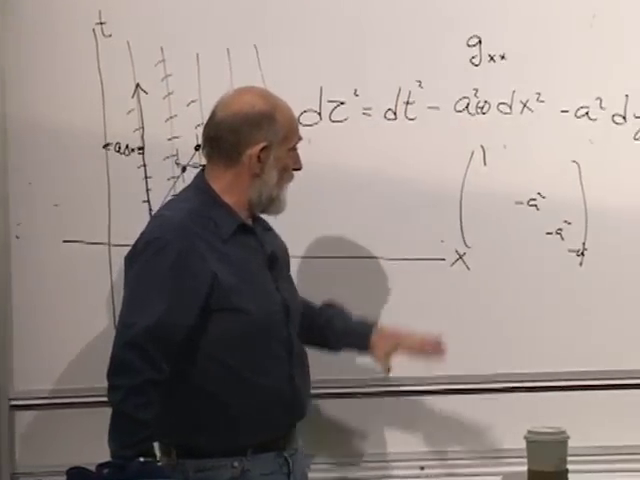
\includegraphics[width=0.82\textwidth]{lecture_01_figure_02.png}
\caption{膨脹的一維宇宙中的共動世界線，以及相應的時空間隔。}
\end{figure}

在三維空間中，同樣的形式可謹慎地推廣為\footnote{黑板上 00:56:38--00:58:51 附近的內容部分被遮住了。這個三維形式是根據講者將一維空間推廣到三維空間的說明，以及黑板上可見的對角形式而寫。}
\begin{equation}
d\tau^2=dt^2-a^2(t)\bigl(dx^2+dy^2+dz^2\bigr),
\end{equation}
度規為對角形式
\begin{equation}
g_{\mu\nu}=\mathrm{diag}\bigl(1,-a^2,-a^2,-a^2\bigr).
\end{equation}
非對角項為零：
\begin{equation}
g_{tx}=g_{ty}=g_{tz}=0.
\end{equation}

均勻性表示度規係數可以依賴時間，但不依賴空間位置。各向同性則表示三個空間方向的形式相同。

\begin{classroomqa}
\audiencequestion{我們不應該把 \(dx\) 視為距離嗎？}\lecturetimestamp{01:01:18}
\lecturerresponse{不。\(dx\)不是距離，\(a\,dx\)才是距離。\(dx\)只是標籤之間的間隔。可以這樣理解：想像有人在某個時刻穿過星系畫出座標網格，並要求網格隨星系移動。座標間隔依照定義保持固定，而物理距離則會改變。也可以把距離單位放進 \(x\)，而不是放進 \(a\)；這只是慣例。重要的是乘積 \(a\,dx\)。}
\end{classroomqa}

\begin{classroomqa}
\audiencequestion{\(dt^2\) 的度規係數等於 \(1\)。這也只是慣例嗎？}\lecturetimestamp{01:03:24}
\lecturerresponse{是的，單就這一點而言並沒有物理意義。如果該係數只依賴時間，就可以改變時間變數，讓它變成單純的 \(dt^2\)。同樣地，也可以選擇使用 \(c=1\) 的單位。這裡不屬於慣例的是：該係數不依賴位置，雖然它可以依賴時間。}
\end{classroomqa}

\begin{classroomqa}
\audiencequestion{如果把它代入愛因斯坦場方程，會得到什麼能量動量張量？}\lecturetimestamp{01:05:59}
\lecturerresponse{那是下一類問題，但屬於動力學，不在目前討論範圍內。可以把這個度規代入愛因斯坦方程，並問什麼樣的能量動量分布能使它成為一個解。這非常重要，但目前討論的是幾何，而不是動力學。}
\end{classroomqa}

\section{視界遮蔽了什麼}

只有在近似的意義下，我們才把大尺度宇宙視為均勻且各向同性。以恆星、行星，甚至單一星系的尺度來看，它顯然並不均勻；局部觀測也不會處處完全各向同性。

農田可以說明這種尺度依賴性。在某個尺度上，農田看起來很規則；尺度小得多時，顯然就不是如此；尺度大於整片農田時，它也不再顯得均勻。宇宙學也是如此。對許多星系取平均後，大尺度分布看起來大致均勻；在足夠小的尺度上則不然。

宇宙比我們看得見的部分更大，也比我們永遠能看見的部分更大。在實際可探測的尺度上，除了局部變化之外，宇宙是各向同性且均勻的。超出這個範圍，就沒有直接的觀測保證。

\begin{classroomqa}
\audiencequestion{你說我們永遠無法真正直接查明。這是否表示或許有間接查明的方法？}\lecturetimestamp{01:10:34}
\lecturerresponse{或許吧。如今多數人的看法是，宇宙在足夠大的尺度上並不均勻，我自己的猜測也一樣。但這個猜測永遠無法驗證：我不會贏，也不會輸。因為基於基本的物理原因，我們無法比現在看得遠太多。這就是視界的存在。}
\end{classroomqa}

\begin{classroomqa}
\audiencequestion{不能利用引力來尋找可觀測範圍以外的質量嗎？}\lecturetimestamp{01:11:53}
\lecturerresponse{不能。遙遠的質量可能只會使我們處於自由落體狀態。即使坐在封閉的房間裡，我們也處於太陽的引力場中並繞著它運行；但若看不到外面，就很難知道太陽就在那裡。只有潮汐力能揭示它的存在；如果引力源足夠遙遠，潮汐效應可能小到無法探測。}
\end{classroomqa}

因此，視界是直接知識的終極屏障。他甚至近乎確信地說，宇宙的體積至少是我們永遠能看見的區域的一千倍，至於這項說法的理由則留待稍後說明。

\section{有界而無邊界}

現在來看閉合幾何。無限直線是開放且無界的。線段則是有界的，意即其範圍有限。有界不表示存在邊界，而是指範圍有限。

有牆的立方體行不通。它違反均勻性，因為靠近牆的人和遠離牆的人並不等價；它也違反各向同性，因為即使是位於中心的人，朝不同方向看到的情況也不同。

圓或球的內部也不行。位於中心的人朝各個方向看到的情況相同，但這種對稱性只存在於一個特殊點。離開中心後，某個方向上的牆較近，另一個方向上的牆較遠。如此一來，一般位置的觀測者所處的空間既不均勻，也不具各向同性。

在極大的尺度上，工作假設是宇宙均勻且各向同性。這就是宇宙學原理。它很有用，但仍可能需要修正。

\begin{classroomqa}
\audiencequestion{處處各向同性是否代表均勻？}\lecturetimestamp{01:18:57}
\lecturerresponse{是。如果每位觀測者朝各個方向看到的情況都相同，就表示空間均勻。但反過來並不成立。均勻本身不代表各向同性。宇宙可以均勻，卻仍有優先方向；例如，若宇宙中充滿了指向同一方向的箭頭，就會如此。}
\end{classroomqa}

合適的有界模型是沒有任何特徵的球面。一個受限於球面上的二維生物，會發現每個位置在局部都和其他位置相同，各個方向也都彼此相同，儘管這個世界是有限的。這就是有界而無邊界。

\section{圓上的閉合一維宇宙}

為了讓代數保持簡單，把球面的例子簡化成一個空間維度：在圓上生活。在一維空間中，各向同性表示左與右等價；圓恰好具有這項特性。選一點作為 \(\theta=0\)。其他各點都以角座標 \(\theta\) 標記，角度以弧度為單位。緊鄰原點一側的點，可以用微小的負角描述，也可以用略小於 \(2\pi\) 的角描述。這種週期性是幾何的一部分。

圓上的居民能接觸到的是圓周，而不是外部的半徑或中心。他們可以沿著圓前進，直到回到原點，以此測量繞行一周的總距離。若把圓畫在周遭的平面上，也可以引入類似半徑的量；但那屬於嵌入圖像，不屬於居民所測量的內在幾何。

這裡的黑板圖很有用，因為角度標記和總周長都呈現在同一幅圖中。
\begin{figure}[H]
\centering
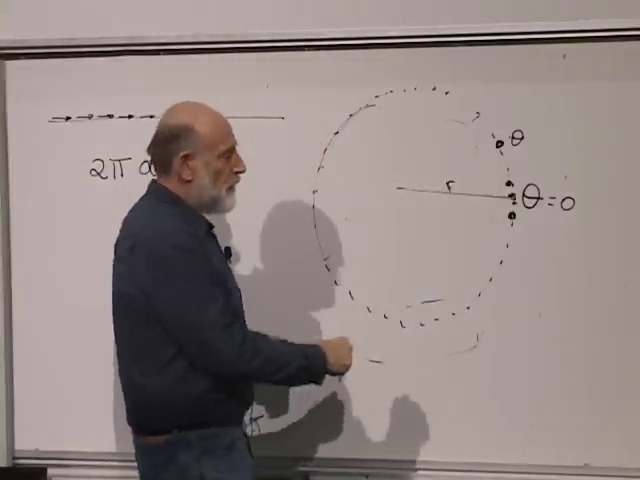
\includegraphics[width=0.82\textwidth]{lecture_01_figure_03.png}
\caption{閉合一維宇宙的角度描述，總周長為 \(2\pi a\)。}
\end{figure}

一種方便的慣例是\footnote{在 01：26：40--01：29：20，記號短暫地在兩種寫法之間切換：一種把整個圓周長直接當作標度因子，另一種則寫成 \(2\pi a\)。這裡採用後一種慣例，因為弧長公式使用的就是這種寫法。}
\begin{equation}
L=2\pi a,
\end{equation}
其中 \(L\) 是總周長。

對於微小的角間隔 \(\Delta\theta\)，物理距離為
\begin{equation}
d=a\,\Delta\theta.
\end{equation}
取無窮小極限可得
\begin{equation}
ds=a\,d\theta,
\end{equation}
因此
\begin{equation}
ds^2=a^2\,d\theta^2.
\end{equation}
這就是圓上的局部度規。

若 \(a\) 隨時間變化，閉合的一維宇宙就會膨脹或收縮。對固定的一對星系而言，
\begin{equation}
d(t)=a(t)\,\Delta\theta,
\end{equation}
因此
\begin{equation}
\dot d=\dot a\,\Delta\theta
      =\frac{\dot a}{a}\,d.
\end{equation}
這裡同樣適用哈勃定律，至少對於間距沒有大到使沿圓的另一側測量產生歧義的星系對而言。

時空度規變成
\begin{equation}
d\tau^2=dt^2-a^2(t)\,d\theta^2.
\end{equation}
若 \(a\) 為常數，時空圖像就是圓柱。若 \(a\propto t\)，圖像就是圓錐。若 \(a(t)\) 的變化較不規則，圖像就會像花瓶。

把圖像倒過來看，星系會彼此越來越接近。若圓周上有 \(360\) 個星系，到了較晚時期，它們會分布得很開；較早時則彼此非常接近，再往前推又會更近。最後，它們不再是彼此分離的星系；再往前推，甚至不再是彼此分離的原子。但空間中仍然沒有任何特殊點。

這就是在此模型中，對「大爆炸發生在哪裡？」這個問題最直接的回答。當 \(a(t)\to 0\) 時，每個間隔 \(a(t)\,\Delta\theta\) 都趨近於零。整個宇宙各處同時收縮。星系並不是從外部空間中的某個特定位置向外飛散；改變尺度的是幾何本身。就這個意義而言，答案是：無所不在。

\begin{classroomqa}
\audiencequestion{你說時空是彎曲的。如果時空是圓柱形，還會是彎曲的嗎？}\lecturetimestamp{01:38:04}
\lecturerresponse{不。如果是圓柱形，就不會是彎曲的。那是 \(a\) 隨時間保持常數的情形。它看起來是彎曲的，只是因為圖像畫在更高維的空間中。把圓柱剪開，就能不經拉伸而攤平。}
\end{classroomqa}

接著討論圓錐。若 \(a\propto t\)，時空圖像就是圓錐。遠離圓錐頂端的部分，在相同的內在意義上也是平坦的：可以把它展開成平面。頂端則不同；那裡是圓錐奇點。

接下來要討論球面宇宙的幾何，以及決定 \(a(t)\) 如何增長或縮小的動力學。
